% \documentclass{beamer}
% \usetheme{Boadilla}

% \title{Thesis}
% \subtitle{Action Recognition and Localization}
% \author{Stathis Galanakis}
% \institute{National University of Athens}
% \date{\today}

% \begin{document}

% \section{\tl{Background}}

% \subsection{\tl{Machine Learning}}

% \begin{frame}
%   \frametitle{Κατηγορίες αλγορίθμων \tl{Machine Learnign}}
% \begin{columns}

% \onslide<2->{  \column{0.5\textwidth}
%   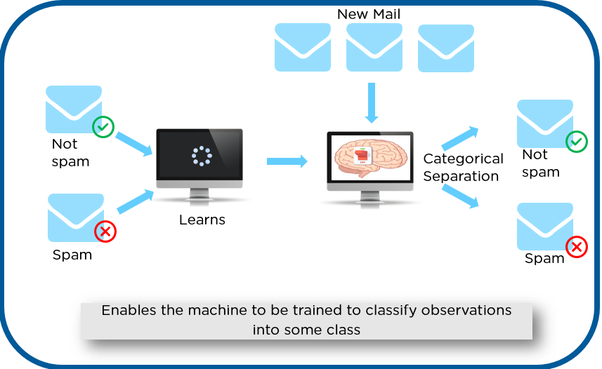
\includegraphics[scale=0.2]{supervised_leaning_example2}
%   \centering
%   \tl{Supervised Learning}
% }
% \onslide<3-> { \column{0.5\textwidth}
%   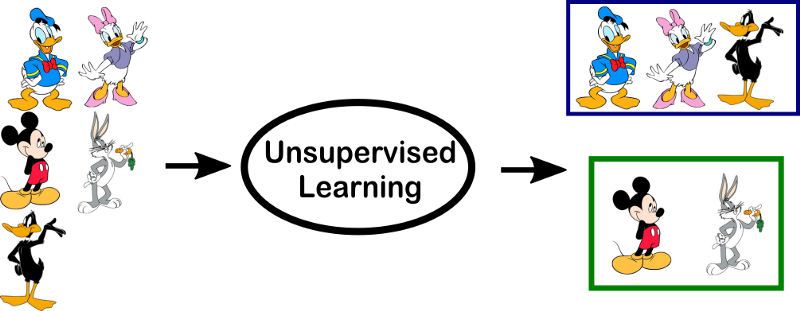
\includegraphics[scale=0.2]{unsupervised_learning_example}
%   \centering
%   \tl{Unsupervised Learning}}
% \end{columns}

% \begin{center}
%   \onslide<4->{
%     \begin{figure}
%       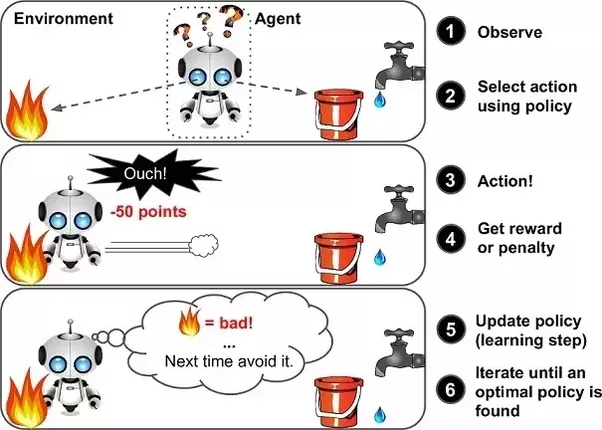
\includegraphics[scale=0.2]{reinforment_learning_example}
%     \end{figure}
%     \tl{Reinforcement Learning}
% }
% \end{center}
% \end{frame}

\subsection{\tl{Object Detectors}}
\begin{frame}
  \frametitle{\tl{Object Detectors}}
  \centering
  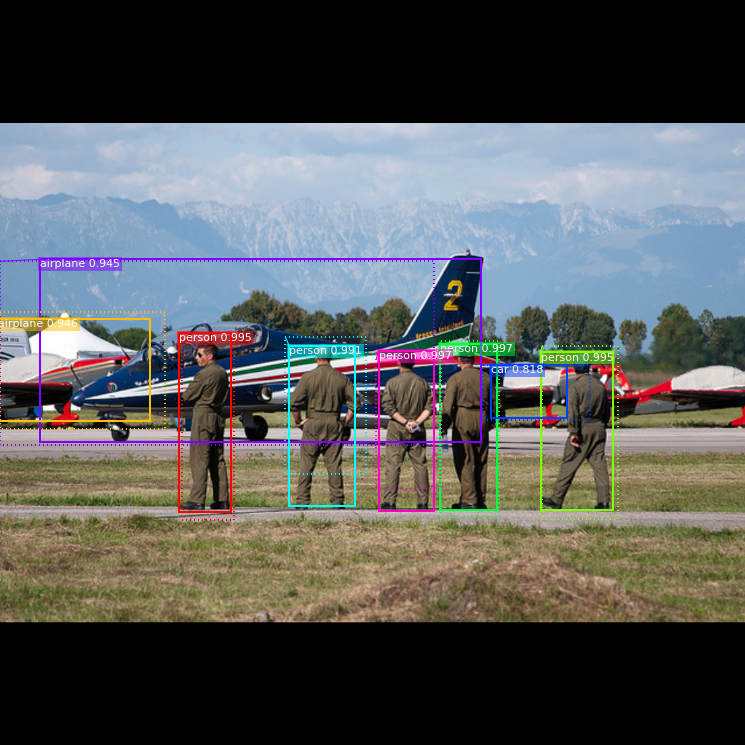
\includegraphics[scale=0.2]{mask_results}
\end{frame}

\begin{frame}
  \frametitle{\tl{Object Detectors}}
\begin{columns}
  \column{0.5\textwidth}
  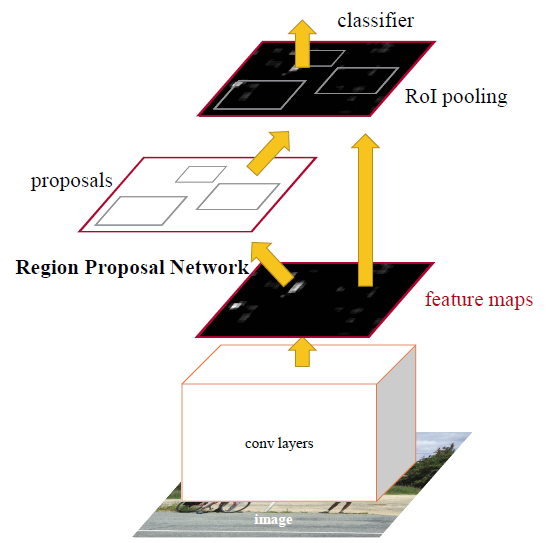
\includegraphics[scale=0.2]{fasterRCNN}
  \centering
  \\
  \tl{Faster R-CNN}

  \column{0.5\textwidth}
  \centering
  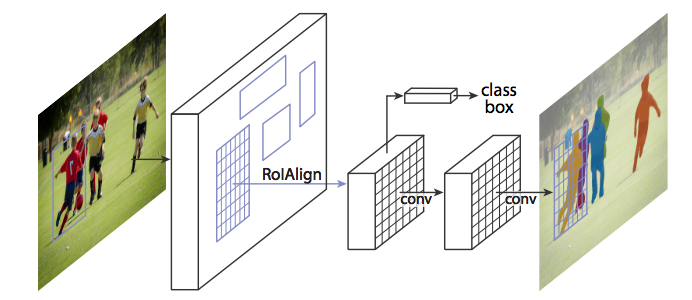
\includegraphics[scale=0.2]{mask_structure}
  \\
  \tl{Mask R-CNN}

\end{columns}
\end{frame}


\begin{frame}
  \frametitle{\tl{Object Detectors}}
\begin{columns}
  \column{0.5\textwidth}
  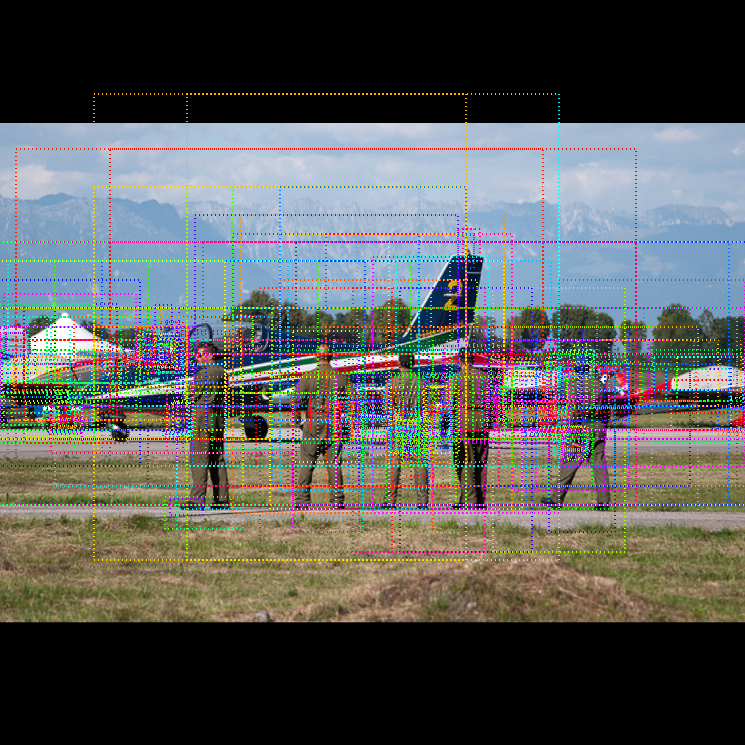
\includegraphics[scale=0.2]{mask_proposals}
  Προτάσεις περιοχών 
  \centering
  \column{0.5\textwidth}
  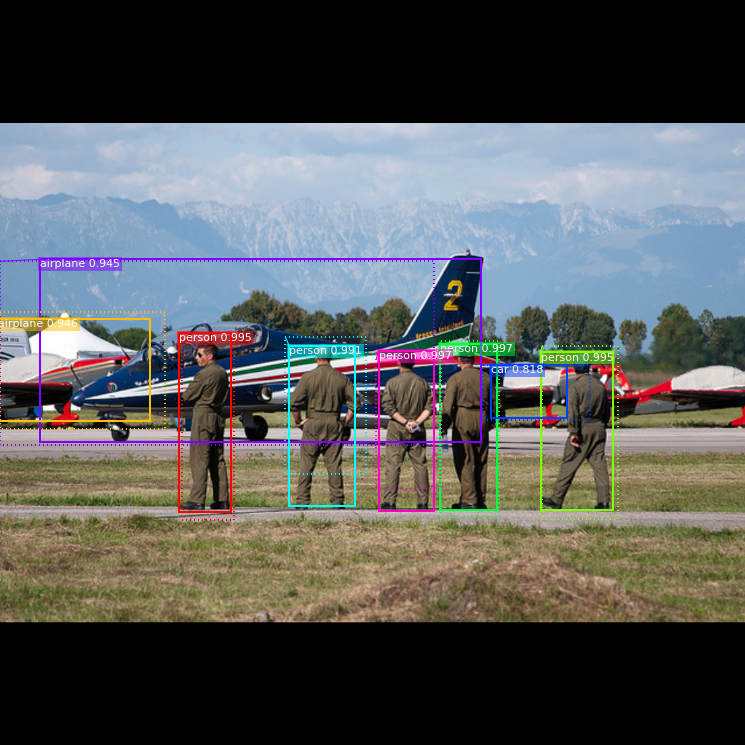
\includegraphics[scale=0.2]{mask_results}
  \centering
  Αποτελέσματα
\end{columns}
\end{frame}
\subsection{\tl{Losses} \gr και \tl{Metrics}}


% \end{document}